



~\\



\begin{minipage}{\linewidth}
\center{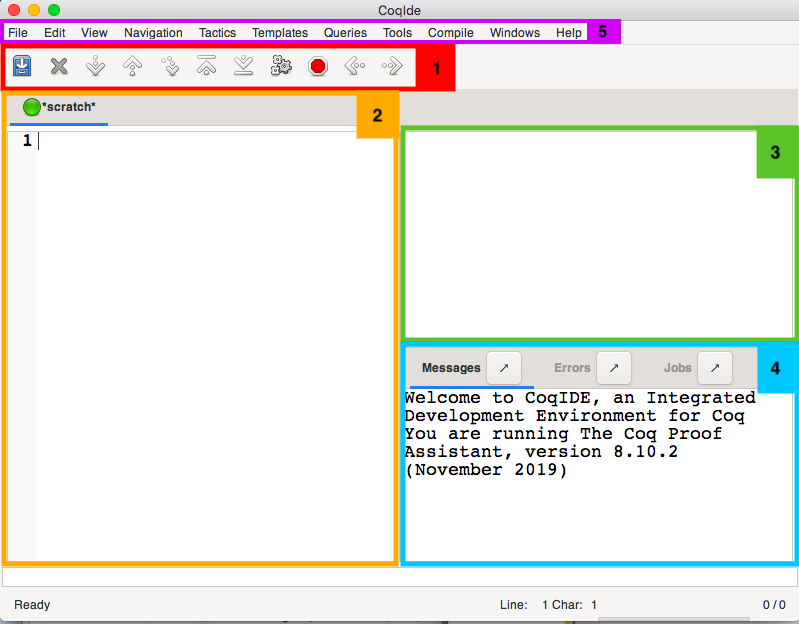
\includegraphics[width=\textwidth]
        {CoqScreenshots/CoqIDEv8_10_2_color.png}}
        \label{fig:IDEcolor} 
        \captionof{figure}{CoqIDE v8.10.2  
        (1) Toolbar. (2) Script Buffer. (3) Goal Window. (4) Message Window. }
\end{minipage}

\subsubsection{Toolbar for CoqIDE v8.10.2}
\hspace{-0.75cm}
\begin{tabular}{ C L }
\centered{
\includegraphics[width=\iconsize]
        {CoqScreenshots/save_10.png}}
        & \centeredl{Save current buffer. 
        If it hasn't been previously saved, functions as save as; use the extension .v to save as a Coq file.
        } \\ \\
\centered{
\includegraphics[width=\iconsize]
        {CoqScreenshots/close_10.png}}
	& \centeredl{Close current buffer. 
	Gives a warning if the file has unsaved changes.
	} \\ \\
\centered{
\includegraphics[width=\iconsize]
        {CoqScreenshots/step_forward_10.png}}
	& \centeredl{Forward one command.
	Steps forward to evaluate the next command in the current file.
	} \\ \\
\centered{
\includegraphics[width=\iconsize]
        {CoqScreenshots/step_backward_10.png}}
	& \centeredl{Backward one command.
	Steps backward one command in the file, returns the state to where it was before evaluating that command. 
	} \\ \\ 
\centered{
\includegraphics[width=\iconsize]
        {CoqScreenshots/go_to_cursor_10.png}}
	& \centeredl{Go to cursor.
	Evaluate all commands in file up to where the cursor currently is.
	} \\ \\ 
\centered{
\includegraphics[width=\iconsize]
        {CoqScreenshots/go_to_top_10.png}}
	& \centeredl{Restart Coq.
	Returns to the top of the file, where no commands have been evaluated.
	} \\ \\ 
\centered{
\includegraphics[width=\iconsize]
        {CoqScreenshots/go_to_bottom_10.png}}
	& \centeredl{Go to end.
	Evaluate to the bottom of the file. 
	Does not work as well with load commands and require import commands.
	} \\ \\
\centered{
\includegraphics[width=\iconsize]
        {CoqScreenshots/check_10.png}}
	& \centeredl{Fully check the document.
	Submits proof terms to the Coq kernel for type checking.
	} \\ \\
\centered{
\includegraphics[width=\iconsize]
        {CoqScreenshots/stop_10.png}}
	& \centeredl{Interrupt computations.
	Stops computation at whatever point was reached before pressing the button.
	} \\ \\
\centered{
\includegraphics[width=\iconsize]
        {CoqScreenshots/next_occurrence_10.png}}
	& \centeredl{Next Occurrence.
	Goes to the next occurrence of whatever the cursor is currently by. 
	Works well for longer words.
	} \\ \\
\centered{
\includegraphics[width=\iconsize]
        {CoqScreenshots/previous_occurrence_10.png}}
	& \centeredl{Previous Occurrence.
	Goes to the previous occurrence of whatever the cursor is currently by.
	Works well for longer words.
	}
\end{tabular}










%\subsection{CoqIDE version 8.7.2}
%	


\begin{minipage}{\linewidth}
\center{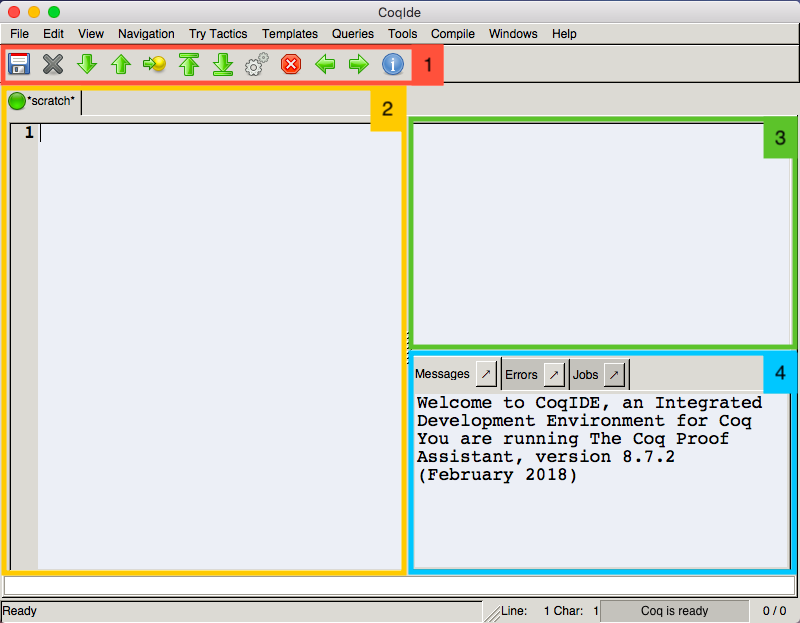
\includegraphics[width=\textwidth]
        {CoqScreenshots/CoqIDE_color.png}}
        \label{fig:IDEcolor} 
        \captionof{figure}{CoqIDE v8.7.2  
        (1) Toolbar. (2) Script Buffer. (3) Goal Window. (4) Message Window. }
\end{minipage}


\subsubsection{Toolbar for CoqIDE v8.7.2}
\hspace{-0.75cm}
\begin{tabular}{ C L }
\centered{
\includegraphics[width=\iconsize]
        {CoqScreenshots/save.png}}
        & \centeredl{Save current buffer. 
        If it hasn't been previously saved, functions as save as; use the extension .v to save as a Coq file.
        } \\ \\
\centered{
\includegraphics[width=\iconsize]
        {CoqScreenshots/close.png}}
	& \centeredl{Close current buffer. 
	Gives a warning if the file has unsaved changes.
	} \\ \\
\centered{
\includegraphics[width=\iconsize]
        {CoqScreenshots/step_forward.png}}
	& \centeredl{Forward one command.
	Steps forward to evaluate the next command in the current file.
	} \\ \\
\centered{
\includegraphics[width=\iconsize]
        {CoqScreenshots/step_backward.png}}
	& \centeredl{Backward one command.
	Steps backward one command in the file, returns the state to where it was before evaluating that command. 
	} \\ \\ 
\centered{
\includegraphics[width=\iconsize]
        {CoqScreenshots/go_to_cursor.png}}
	& \centeredl{Go to cursor.
	Evaluate all commands in file up to where the cursor currently is.
	} \\ \\ 
\centered{
\includegraphics[width=\iconsize]
        {CoqScreenshots/go_to_top.png}}
	& \centeredl{Restart Coq.
	Returns to the top of the file, where no commands have been evaluated.
	} \\ \\ 
\centered{
\includegraphics[width=\iconsize]
        {CoqScreenshots/go_to_bottom.png}}
	& \centeredl{Go to end.
	Evaluate to the bottom of the file. 
	Does not work as well with load commands and require import commands.
	} \\ \\
\centered{
\includegraphics[width=\iconsize]
        {CoqScreenshots/check.png}}
	& \centeredl{Fully check the document.
	Submits proof terms to the Coq kernel for type checking.
	} \\ \\
\centered{
\includegraphics[width=\iconsize]
        {CoqScreenshots/stop.png}}
	& \centeredl{Interrupt computations.
	Stops computation at whatever point was reached before pressing the button.
	} \\ \\
\centered{
\includegraphics[width=\iconsize]
        {CoqScreenshots/next_occurrence.png}}
	& \centeredl{Next Occurrence.
	Goes to the next occurrence of whatever the cursor is currently by. 
	Works well for longer words.
	} \\ \\
\centered{
\includegraphics[width=\iconsize]
        {CoqScreenshots/previous_occurrence.png}}
	& \centeredl{Previous Occurrence.
	Goes to the previous occurrence of whatever the cursor is currently by.
	Works well for longer words.
	} \\ \\
\centered{
\includegraphics[width=\iconsize]
        {CoqScreenshots/proof_wizard.png}}
	& \centeredl{Proof Wizard. 
	Tries to apply a given set of tactics in order. 
	The tactics to be attempted can be customized by going to: 
	Edit tab $\to$ Preferences, then select Tactics Wizard in the leftmost pane of the Customizations window.} 
\end{tabular}











\newpage
\subsection{Script Buffer}
Here you can type out new definitions and proofs in a new buffer, or open a buffer from a saved file by going to the File tab $\to$ Open, then choosing the file. 
You can edit and save new and existing buffers here. 
\begin{code} 
	This block represents a script buffer in this tutorial. 
\end{code}



\subsection{Goal Window}
Goals to be proven will be displayed here. 
This window will be empty unless you're in a proof environment; inside the proof environment, it will display what you goal are currently proving, what goals are left to be proved, or that there are no more subgoals and your proof is complete.
\begin{goal} 
	This block represents the goal window in this tutorial. 
\end{goal}



\subsection{Message Window}
Any messages resulting from an executed command will be displayed here. 
Results from queries are also printed out here. 
Clicking the arrow in the corner of the Messages, Errors, or Jobs tab here will create a separate window for that tab. 
When the separate window is closed, it will return to the main Coq IDE window. 
\begin{msg} 
	This block represents the message window in this tutorial. 
\end{msg}






\subsection{Menu Bar}

\paragraph{\underline{File}}
~\\
\TT{New} : Open a new blank scratch buffer (for writing definitions and proving in Coq)
\\
\TT{Open} : Open a file stored in memory
\\
\TT{Save} : Save your current file. Functions as \TT{Save as} when used on an unsaved scratch buffer. 
\\ 
\TT{Save as} : Opens a pop-up window to choose where to save the current buffer and give it a name. 
\\
\TT{Revert all buffers} : Likely intended to undo changes in all buffers, back to previously saved state 
	(Currently seems to have no effect).  % ? Seems to have no effect when clicked.
\\
\TT{Close buffer} : Close the current buffer. Will give a warning if you have unsaved changes. 
\\
\TT{Print} : Shows you the command to use in the command line to print the current buffer file. 
\\
\TT{Export to} : Allows you to export the current file as a file of a different type. 
	\\ \-\ \qquad Options: Html, LaTeX, Dvi, Pdf, Ps
\\
\TT{Rehighlight} : Rehighlight text. % ? Seems to have no effect when clicked.
\\
\TT{Quit} : Close the CoqIDE. Will give a warning if there are unsaved changes. 





~\\
\paragraph{\underline{Edit}}
~\\
\TT{Undo} : Undo last typing action
\\
\TT{Redo} : Redo last typing action removed by \TT{Undo}
\\
\TT{Cut} : Cut text. Can be pasted into other programs. 
\\
\TT{Copy} : Copy text. Can be pasted into other programs.
\\ 
\TT{Paste} : Paste copied text. Works with text copied from other programs, but can lose characters (i.e., \_)
\\
\TT{Find / Replace} : Opens a window to find text (and replace if desired). 
	Can be detached to be in its own window separate from the main CoqIDE. 
\\
\TT{Find Next} : Go to next occurrence.  %? Seemingly not working. 
\\
\TT{Find Previous} : Go to previous occurrence.  %? Seemingly not working. 
\\
\TT{External editor} : Looks for and attempts to load a \TT{.aux} file of the same name as the current buffer. 
	Prints results in \TT{Message} window. 
\\
\TT{Preferences} : Pop up window to modify your preferences for the CoqIDE 
(i.e., customize font, font size, editor configurations, colors, etc.)





~\\
\paragraph{\underline{View}}
~\\
\TT{Previous tab} : Move to the buffer in the tab before the current one (can also click on the tab of the desired buffer). 
\\
\TT{Next tab} : Move to the buffer in the tab after the current one (can also click on the tab of the desired buffer).
\\
\TT{Zoom in} : Increase the size of the text in the buffer, messages, and goal window (affects all buffers).  
\\
\TT{Zoom out} : Decrease the size of the text in the buffer, messages, and goal window (affects all buffers).  
\\
\TT{Zoom fit} : Intended to return to normal zoom level % ? Doesn't seem to have an affect currently.
\\
\TT{Show Toolbar} : Toggle to show/hide toolbar (toolbar discussed in subsection \ref{subsec: toolbar}). 
\\
\TT{Query Pane} : Shows/hides the query pane (appears across the bottom of the CoqIDE). 
	Can be detached into its own window. 
\\
\TT{Display implicit arguments} : 
\\
\TT{Display coercions} : 
\\
\TT{Display raw matching expressions} : 
\\
\TT{Display notations} : 
\\
\TT{Display all basic low-level contents} : 
\\
\TT{Display existential variable instances} : 
\\
\TT{Display universe levels} : 
\\
\TT{Display all low-level contents} : 
\\
\TT{Display unfocused goals} : 
\\
\TT{Don't show diffs}, \TT{Show diffs:only added}, \TT{Show diffs:added and removed} : Choices for displaying diffs (must choose from one of the three)

	
	
	
~\\
\paragraph{\underline{Navigation}}
~\\
Note: these are like their toolbar button equivalents. 
Please see the subsection \ref{subsec: toolbar} for further descriptions given there. 
\\
\TT{Forward} : Forward one command. 
\\ 
\TT{Backward} : Backward one command. 
\\
\TT{Go to} : Go to cursor. 
\\
\TT{Start} : Restart Coq. 
\\
\TT{End} : Go to end. 
\\
\TT{Interrupt} : Interrupt computations. 
\\
\TT{Previous} : Previous Occurrence. 
\\
\TT{Next} : Next Occurrence. 




	
~\\
\paragraph{\underline{Tactics}}
Places tactics that can be used in proofs at the cursor location in the current buffer. 
Some of these are discussed in further detail in Section \ref{Sec: tactics}; 
all can be found in the \href{https://coq.inria.fr/distrib/V8.10.2/refman/coq-tacindex.html}{online documentation}. 
~\\
\TT{a...} : Places the given tactic. Includes options: 
	\TT{abstract}, \TT{absurd}, \TT{apply}, \TT{apply \_ with}, \TT{assert}, \TT{assert (\_:\_)}, 
	\TT{assert (\_:=\_)}, \TT{assumption}, \TT{auto}, \TT{auto with}, \TT{autorewrite}. 
\\
\TT{c...} : Places the given tactic. Includes options: 
	\TT{case}, \TT{case \_ with}, \TT{casetype}, \TT{cbv}, \TT{cbv in}, \TT{change}, \TT{change \_ in}, 
	\TT{clear}, \TT{clearbody}, \TT{cofix}, \TT{compare}, \TT{compute}, \TT{compute in}, \TT{congruence}, 
	\TT{constructor}, \TT{constructor \_ with}, \TT{contradiction}, \TT{cut}, \TT{cutrewrite}. 
\\
\TT{d...} : Places the given tactic. Includes options: 
	\TT{decide equality}, \TT{decompose}, \TT{decompose record}, \TT{decompose sum}, 
	\TT{dependent inversion}, \TT{dependent inversion \_ with}, \TT{dependent inversion\_clear}, 
	\TT{dependent inversion\_clear \_ with}, \TT{dependent rewrite ->}, \TT{dependent rewrite <-}, 
	\TT{destruct}, \TT{discriminate}, \TT{do}, \TT{double induction}. 
\\
\TT{e...} : Places the given tactic. Includes options: 
	\TT{eapply}, \TT{eauto}, \TT{eauto with}, \TT{eexact}, \TT{elim}, \TT{elim \_ using}, 
	\TT{elim \_ with}, \TT{elimtype}, \TT{exact}, \TT{exists}. 
\\
\TT{f...} : Places the given tactic. Includes options: 
	\TT{fail}, \TT{field}, \TT{first}, \TT{firstorder}, \TT{firstorder using}, \TT{firstorder with}, 
	\TT{fix}, \TT{fix \_ with}, \TT{fold}, \TT{fold \_ int}, \TT{functional induction}. 
\\
\TT{g...} : Places the given tactic. Includes options: 
	\TT{generalize}, \TT{generalize dependent}. 
\\
\TT{hnf} : Replaces the current goal with its head normal form. 
\\
\TT{i...} : Places the given tactic. Includes options: 
	\TT{idtac}, \TT{induction}, \TT{info}, \TT{injection}, \TT{instantiate (\_:=\_)}, \TT{intro}, 
	\TT{intro after}, \TT{intro \_ after}, \TT{intros}, \TT{intros until}, \TT{intuition}, 
	\TT{inversion}, \TT{inversion \_ in}, \TT{inversion \_ using}, \TT{inversion \_ using \_ in}, 
	\TT{inversion\_clear}, \TT{inversion\_clear \_ in}.  
\\
\TT{j...} : Places the given tactic. Includes options: 
	\TT{jp <n>}, \TT{jp}. 
\\
\TT{l...} : Places the given tactic. Includes options: 
	\TT{lapply}, \TT{lazy}, \TT{lazy in}, \TT{left}. 
\\
\TT{move ... after} : Moves the hypothesis named in \TT{...} after the hypothesis given beyond 
	\TT{after} in the local context. 
\\
\TT{omega} : Automatic decision procedure for Presburger arithmetic. 
	Must be loaded using command \TT{Require Import Omega} before use. 
\\
\TT{p...} : Places the given tactic. Includes options: 
	\TT{pattern}, \TT{pose}, \TT{pose \_:=\_)}, \TT{progress}. 
\\
\TT{quote} : The quote plugin was removed, documentation no longer includes information on this tactic. 
\\
\TT{r...} : Places the given tactic. Includes options: 
	\TT{red}, \TT{red in}, \TT{refine}, \TT{reflexivity}, \TT{rename \_ into}, \TT{repeat}, 
	\TT{replace \_ with}, \TT{rewrite}, \TT{rewrite \_ in}, \TT{rewrite <-}, 
	\TT{rewrite <- \_ in}, \TT{right}, \TT{ring}. 
\\
\TT{s...} : Places the given tactic. Includes options: 
	\TT{set}, \TT{set (\_:=\_)}, \TT{setoid\_replace}, \TT{setoid\_rewrite}, \TT{simpl}, 
	\TT{simpl \_ in}, \TT{simple destruct}, \TT{simple induction}, \TT{simple inversion}, 
	\TT{simplify\_eq}, \TT{solve}, \TT{split}, \TT{subst}, \TT{symmetry}, \TT{symmetry in}. 
\\
\TT{t...} : Places the given tactic. Includes options: 
	\TT{tauto}, \TT{transivity}, \TT{trivial}, \TT{try}. 
\\
\TT{u...} : Places the given tactic. Includes options: 
	\TT{unfold}, \TT{unfold \_ in}.  






	
~\\
\paragraph{\underline{Templates}}
Places the selected item in the current buffer at the cursor's location. 
Gives the most commonly desired items at top, and others within multi-option menus. 
~\\
\TT{Lemma} : Places the template for a new lemma. 
\\
\TT{Theorem} : Places the template for a new theorem. 
\\
\TT{Definition} : Places the template for a new definition. 
\\
\TT{Inductive} : Places the template for a new inductive definition. 
\\
\TT{Fixpoint} : Places the template for a new fixpoint definition. 
\\
\TT{Scheme} : Places the template for a new scheme. 
\\
\TT{match} : Places the template for pattern matching using \TT{match}. 
	Requires this to be inside an inductive type (doesn't seem to be working properly). 
\\
\TT{A...} : Places the given text. Options: 
	\TT{Add Abstract Ring A Aplus Amult Aone Azero Ainv Aeq T.}, 
	\TT{Add Abstract Semi Ring A Aplus Amult Aone Azero Aeq T.}, 
	\TT{Add Field}, \TT{Add LoadPath}, \TT{Add ML Path}, \TT{Add Morphism}, 
	\TT{Add Printing Constructor}, \TT{Add Printing If}, \TT{Add Printing Let}, 
	\TT{Add Printing Record}, \TT{Add Rec LoadPath}, \TT{Add Rec ML Path}, 
	\TT{Add Ring A Aplus Amult Aone Azero Ainv Aeq T [ c1 ... cn ].  }, 
	\TT{Add Semi Ring A Aplus Amult Aone Azero Aeq T [ c1 ... cn ].}, 
	\TT{Add Relation}, \TT{Add Setoid}, \TT{Axiom}. 
\\
\TT{C...} : Places the given text. Options: 
	\TT{Canonical Structure}, \TT{Chapter}, \TT{Coercion}, \TT{Coercion Local}, 
	\TT{CoFixpoint}, \TT{CoInductive}. 
\\
\TT{D...} : Places the given text. Options: 
	\TT{Declare ML Module}, \TT{Defined.}, \TT{Definition}, \TT{Derive Dependent Inversion}, 
	\TT{Derive Dependent Inversion\_clear}, \TT{Derive Inversion}, \TT{Derive Inversion\_clear}.
\\
\TT{E...} : Places the given text. Options: 
	\TT{End}, \TT{End Silent.}, \TT{Eval}, \TT{Extract Constant}, \TT{Extract Inductive}, 
	\TT{Extraction Inline}, \TT{Extraction Language}, \TT{Extraction NoInline}. 
\\
\TT{F...} : Places the given text. Options: 
	\TT{Fact}, \TT{Fixpoint}, \TT{Focus}. 
\\
\TT{G...} : Places the given text. Options: 
	\TT{Global Variable}, \TT{Goal}, \TT{Grammar}. 
\\
\TT{H...} : Places the given text. Options: 
	\TT{Hint}, \TT{Hint Constructors}, \TT{Hint Extern}, \TT{Hint Immediate}, 
	\TT{Hint Resolve}, \TT{Hint Rewrite}, \TT{Hint Unfold}, \TT{Hypothesis}. 
\\
\TT{I...} : Places the given text. Options: 
	\TT{Identity Coercion}, \TT{Implicit Arguments}, \TT{Inductive}, \TT{Infix}. 
\\
\TT{L...} : Places the given text. Options: 
	\TT{Lemma}, \TT{Load}, \TT{Load Verbose}, \TT{Local}, \TT{Ltac}. 
\\
\TT{M...} : Places the given text. Options: 
	\TT{Module}, \TT{Module Type}, \TT{Mutual Inductive}. 
\\
\TT{N...} : Places the given text. Options: 
	\TT{Notation}, \TT{Next Obligation}. 
\\
\TT{O...} : Places the given text. Options: 
	\TT{Opaque}, \TT{Obligations Tactic}. 
\\
\TT{P...} : Places the given text. Options: 
	\TT{Parameter}, \TT{Proof.}, \TT{Program Definition}, \TT{Program Fixpoint}, 
	\TT{Program Lemma}, \TT{Program Theorem}. 
\\
\TT{Qed} : Places the \TT{Qed.} command for completing a proof. 
\\
\TT{R...} : Places the given text. Options: 
	\TT{Read Module}, \TT{Record}, \TT{Variant}, \TT{Remark}, \TT{Remove LoadPath}, 
	\TT{Remove Printing Constructor}, \TT{Remove Printing If}, \TT{Remove Printing Let}, 
	\TT{Remove Printing Record}, \TT{Require}, \TT{Require Export}, \TT{Require Import}, 
	\TT{Reset Extraction Inline}, \TT{Restore State}. 
\\
\TT{S...} : Places the given text. Options: 
	\TT{Scheme}, \TT{Section}, \TT{Set Extraction AutoInline}, \TT{Set Extraction Optimize}, 
	\TT{Set Hyps\_limit}, \TT{Set Implicit Arguments}, \TT{Set Printing Wildcard}, \TT{Set Silent.}, 
	\TT{Set Undo}, \TT{Structure}, \TT{Syntactic Definition}, \TT{Syntax}. 
\\
\TT{T...} : Places the given text. Options: 
	\TT{Test Printing If}, \TT{Test Printing Let}, \TT{Test Printing Synth}, \TT{Test Printing Wildcard}, 
	\TT{Theorem}, \TT{Time}, \TT{Transparent}. 
\\
\TT{U...} : Places the given text. Options: 
	\TT{Unfocus}, \TT{Unset Extraction AutoInline}, \TT{Unset Extraction Optimize}, 
	\TT{Unset Hyps\_limit}, \TT{Unset Implicit Arguments}, \TT{Unset Printing Wildcard}, 
	\TT{Unset Silent.}, \TT{Unset Undo}. 
\\
\TT{V...} : Places the given text. Options: 
	\TT{Variable}, \TT{Variables}. 
\\
\TT{Write State} : Places the given text. 





	
~\\
\paragraph{\underline{Queries}}
~\\
These are described and have examples of their use in section \ref{Sec: queries}. 
\\
\TT{Search} : See subsection \ref{search}. 
\\
\TT{Check} : See subsection \ref{check}. 
\\
\TT{Print} : See subsection \ref{print}. 
\\
\TT{About} : See subsection \ref{about}. 
\\
\TT{Locate} : See subsection \ref{locate}. 
\\
\TT{Print Assumptions} : See subsection \ref{print_assumptions}. 



	
~\\
\paragraph{\underline{Tools}}
~\\
\TT{Comment} : Comments out highlighted text. 
	Will wrap another commented out layer around currently commented out text. 
\\ 
\TT{Uncomment} : Uncomments highlighted text. If not commented out, no effect. 
\\
\TT{Coqtop arguments} : Opens a separate window with the Coq command for this. 
\\
\TT{LaTeX-to-unicode} : Likely used to convert text in file from LaTeX to unicode. 





	
~\\
\paragraph{\underline{Compile}}
~\\
\TT{Compile buffer} : Compiles the current buffer, creates a \TT{.glob} file and a \TT{.vo} file. 
\\
\TT{Make} : Looks for a makefile and runs it if found. 
	Compiles the buffers included in the makefile as the above command would, 
	and creates \TT{.aux} files for each. 
\\
\TT{Next error} : Go to next error, if there is one. % doesn't always seem to work
\\
\TT{Make makefile} : Creates a makefile (\TT{makefile}) for the current directory, 
	and a makefile configuration file (\TT{makefile.conf}). Can then be run using the \TT{Make} 
	command from above. Has a \TT{make clean} command to clean up after the make if desired. 
 




	
~\\
\paragraph{\underline{Windows}}
~\\
\TT{Detach view} : Pops out the goal window into its own separate window. 
	To move it back to the IDE window, close the detached window. 




	
~\\
\paragraph{\underline{Help}}
~\\
\TT{Browse Coq Manual} : Online reference manual. Opens \url{https://coq.inria.fr/distrib/V8.10.2/refman/}
\\ 
\TT{Browse Coq Library} : Online standard library. Opens \url{https://coq.inria.fr/distrib/V8.10.2/stdlib/}
\\
\TT{Help for keyword} : Searches for highlighted keyword 
	(Doesn't find the documentation well - websites are much more useful). 
\\
\TT{Help for $\mu$PG mode} : Prints out help for this mode (for use with Emacs, I believe) in the \TT{Message} window.
\\ 
\TT{About} : Pop-up window giving info about current CoqIDE.



















